\centerline{\bf I. Introduction}
\addcontentsline{toc}{subsection}{I. Introduction}
\smallskip

\rory{get 'er done!}

\bigskip
\centerline{\bf II. Objectives and Significance}
\addcontentsline{toc}{subsection}{II. Objectives and Significance}
\smallskip

\bigskip
\centerline{\bf III. Team Qualifications and Previous NASA Support}
\addcontentsline{toc}{subsection}{III. Team Qualifications and Previous NASA Support}
\smallskip

\bigskip
\centerline{\bf IV. Technical Approach and Methodology}
\addcontentsline{toc}{subsection}{IV. Technical Approach and Methodology}
\smallskip

\section{Transit Duration}

\begin{eqnarray}
\Delta t_{circ} & = & {{P}\over{\pi}}~{{\sqrt{R_*^2 - b_0^2}}\over{a}} \nonumber \\
                & = & {{P}\over{\pi}}~{{\sqrt{1 - bRs_0^2}}\over{aRs}}
\label{eq-tcirc}
\end{eqnarray}
where $P$ is the orbital period in cgs units, $R_*$ the stellar radius
in cgs, $b_0$ the minimum planetary impact parameter in cgs, $bRs_0$ a
unitless measure of the minimum impact parameter (scaled by the stellar
radius), $a$ the planetary semi--major axis in cgs, and $aRs$ this
value scaled by the stellar radius.

\section{Fitted Transit Model}
To avoid a circular dependency between the fitted model and a physical
model that includes orbital dynamics, we parameterize the fitted
lightcurve in purely geometric terms.  To do so, we adopt the
quadratic limb--darkened model of \cite{2002ApJ...580L.171M}, which
describes transit lightcurves in terms of two (nuisance)
limb--darkening coefficients and two (important) system parameters.
The first of the system parameters is the planetary radius divided by
the stellar radius (${\bf rRs = Rp/R_*}$), which determines the
fractional area of the stellar disk that may be occulted by the
planet.  The second is the impact parameter of the planet (${\bf bRs =
  b/R_*}$).  This variable is a function of time due to the objects'
relative motion.  This function is dependent on the chord that the
planet takes across the stellar disk, itself typically estimated using
the orbital parameters semi--major axis and inclination.  

%However, since we wish to determine the transit durations in the
%absence of any assumptions about the orbital dynamics, and to compare
%the {\it measured} durations to the {\it expected} durations in the
%cases of circular orbits, we cannot represent the time--dependent
%impact parameter as such.

Instead we use here a purely geometric parameterization, represented
in Figure~\ref{fig-schem}.  We describe the impact parameter as a
function of time using the minimum impact parameter ${\bf bRs_0}$ --
when the centers of the sources are aligned along the x--axis at
center--of--transit time ${\bf t_0}$ -- and the location of the planet
on the transit chord across the stellar disk.  The x--coordinate of
the planet as a function of time is represented as ${\bf x(t) / R_* =
  (t - t_0) * v_\perp / R_* = (t - t_0) / tRs}$, where ${\bf v_\perp}$
is the unknown perpendicular velocity, and ${\bf tRs}$ is the amount
of time it takes the planet to traverse the stellar radius.  This
allows us to express the impact parameter as a function of time as:

\begin{eqnarray}
bRs(t) & = & \sqrt{bRs_0^2 + \left((t - t_0) / tRs\right)^2}
\end{eqnarray}

The transit duration ${\bf \Delta t}$ may be found from the 2
solutions to ${\bf bRs(t) = 1}$, and represents the time between the
center of the planet crossing each limb of the star:

\begin{eqnarray}
\Delta t & = & 2 * tRs \sqrt{1 - bRs_0^2}.
\label{eq-dt}
\end{eqnarray}


This model yields a 4--parameter fit to each transit in ${\bf t_0,
  bRs_0^2, tRs, rRs}$.

\section{Fake Lightcurve Generation}

{\bf RORY} Describe the fake systems

We use the system inclination, semi--major axis, planet--to--star
radius ratio, and period (along with two limb darkening parameters) to
generate fake system lightcurves using the method of
\cite{2002ApJ...580L.171M}.  The system lightcurve is evaluated once
each minute and integrated over 30 evaluations to approximate a single
Kepler long--cadence observation.  This is done for a window of 1 day
on either side of the given transit midpoint to ensure significant
out--of--transit data to include in the fit.  We perform these
evaluations for all transits for 14 ``quarters'' of Kepler
observations, or approximately 1280 days.

A white--noise component is added to each lightcurve for each of 4
magnitude bins, using the precisions in parts--per--million (ppm)
given on the Kepler calibration
webpage \footnote{http://keplergo.arc.nasa.gov/CalibrationSN.shtml}.
We evaluate each lightcurve separately for magnitude 8/10/12/14
objects, adding a random contribution of amplitude 11.3/29/80/296 ppm
(respectively) to each datapoint as generated above.  We do not
include red noise, or other transient gaps and features known to exist
in the Kepler data.  This yields a set of 4 lightcurves per simulated
system, each having hundreds of individual transits to fit.

\section{Model Fitting}

To examine how our knowledge of system parameters evolves as a
function of number of transits, we model each transit separately.
I.e. for transit $i$ we have model parameters ${\rm t_{0;i},
  bRs_{0;i}^2, tRs_i, rRs_i}$.  If we do not expect any evolution in
the system parameters we may instead fit common terms across transits,
i.e. for transits $1...N$ we have model parameters ${\rm t_{0;1},
  t_{0;2}, ..., t_{0;N}, bRs_0^2, tRs, rRs}$ for a total of N+3
parameters.  However, since we wish to examine our model sensitivity
as a function of system brightness and number of transits, we model
each transit separately, and combine the parameter constraints from
each step after the fact.

We do this by using the affine--invariant MCMC sampler {\tt emcee}
\citep{2013PASP..125..306F} to provide posterior distributions of the
model parameters.  This provides a set of MCMC chains for each transit
that may be combined to yield the posterior distribution of
parameters: i.e. for transit $j$ our knowledge of ${\rm rRs}$ comes
from ${\rm rRs_j = \prod_{i=1}^j rRs_i}$.  We combine the posterior
chains to determine our constraints on common fitted terms ${\rm rRs,
  bRs_0}$ and derived term ${\rm \Delta t}$ via Equation~\ref{eq-dt}.
We use the median and interquartile--range (multiplied by 0.741 to
approximate a Gaussian sigma) of each distribution to estimate the
value best supported by the data, and its uncertainty.  By doing this
in a loop over system brightness $m$, and transit number $n$, we are
able to generate an understanding of how the uncertainty on each
parameter scales with $m$ and $n$.  Importantly, this will inform us
how many of the KOI systems we are able to use in our analysis.

We estimate the period for the system using the ensemble of ${\rm
  t_{0;i}}$ fit to a linear ephemeris, whose posterior we also
determine using {\tt emcee}.  In this manner we are able to provide
posterior distributions for the system parameters of interest: period,
minimum impact parameter, and planetary radius normalized by the
stellar radius.  However, to determine the circular--orbit transit
duration we require an additional parameter: the semi--major axis in
units of the stellar radius ${\rm aRs}$ (Equation~\ref{eq-tcirc}).

\begin{figure*}[t] 
\begin{center} 
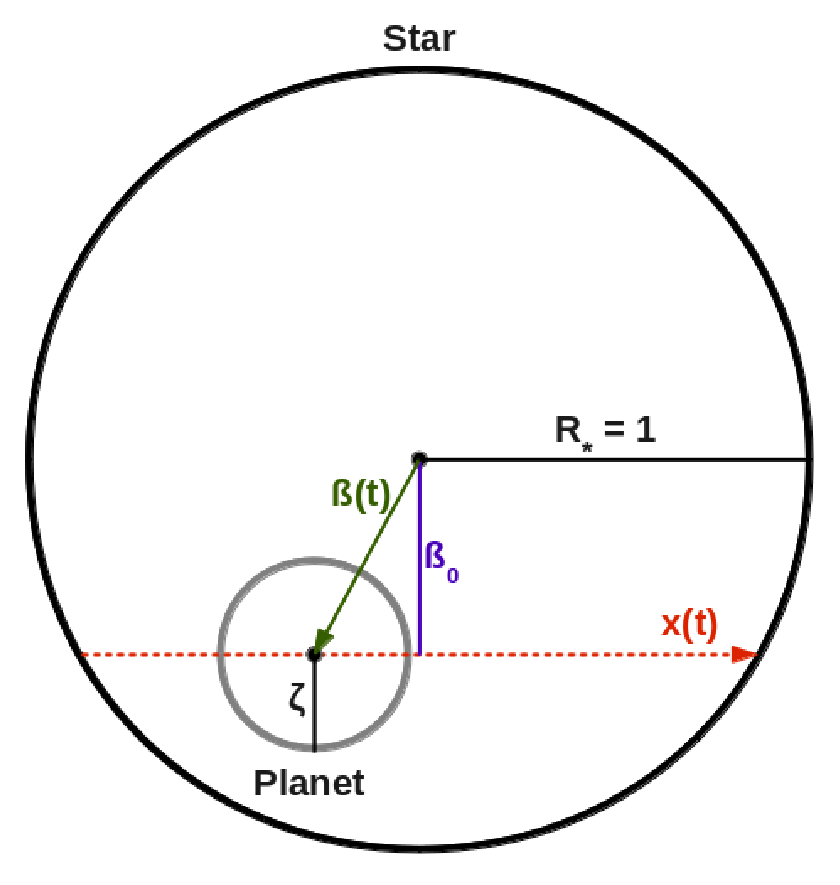
\epsfig{file=figures/schem.eps, width=0.4\textwidth} 
\caption{Schematic}
\label{fig-schem} 
\end{center} 
\end{figure*}

\bigskip
\centerline{\bf V. Broader Impacts}
\addcontentsline{toc}{subsection}{V. Broader Impacts}
\smallskip

This is more relevant for NSF

\bigskip
\centerline{\bf VI. Relevance to NASA Programs}
\addcontentsline{toc}{subsection}{VI. Relevance to NASA Programs}
\smallskip

\bigskip
\centerline{\bf VII. Project Development Plan}
\addcontentsline{toc}{subsection}{VII. Project Development Plan}
\smallskip

\bigskip
\centerline{\bf VIII. Data Sharing Plan}
\addcontentsline{toc}{subsection}{VIII. Data Sharing Plan}
\smallskip
